%----------------------------------------------------------------------------------------
%	PACKAGES AND DOCUMENT CONFIGURATIONS
%----------------------------------------------------------------------------------------

\documentclass[11pt]{article}

\usepackage{graphicx} % Required for the inclusion of images
\usepackage{natbib} % Required to change bibliography style to APA
\usepackage{amsmath} % Required for some math elements 
\usepackage{subcaption}
\usepackage[nomarkers,figuresonly]{endfloat}
\usepackage[margin=0.9in]{geometry}
\usepackage{sectsty}
\sectionfont{\fontsize{12}{15}\selectfont}
\setlength\parindent{0pt} % Removes all indentation from paragraphs

\renewcommand{\labelenumi}{\alph{enumi}.} % Make numbering in the enumerate environment by letter rather than number

%%%%%%%%%% Start TeXmacs macros
\newcommand{\nocomma}{}
\newcommand{\noplus}{}
\newcommand{\tmop}[1]{\ensuremath{\operatorname{#1}}}
\newcommand{\upl}{+}
%%%%%%%%%% End TeXmacs macros

%----------------------------------------------------------------------------------------
%	DOCUMENT INFORMATION
%----------------------------------------------------------------------------------------

\title{ Machine Translation Assignment 2 : Decoding} % Title

\author{s0907677, s152582} % Author name

\date{}

\begin{document}

\maketitle % Insert the title, author and date

%----------------------------------------------------------------------------------------
%	Q 1
%----------------------------------------------------------------------------------------
\section*{Q1}
The default limitation of both stack size and maximum number of translation to 1 is very restrictive and so one expects to see a significant improvement in total log probability once either limit is increased. This proves to be true, but only in a very limited range for both variables.

Changing the maximum number of translations from 1 to 2 leads to a relatively sharp improvement, which flattens out very quickly. The difference in total log probability between decoder with k=10 and k=50 is only 10\% of the difference between k=1 and k=2. No further improvements are observed for k>50.

Changing the stack size has a similar effect, although improvement tapers out even quicker. Increasing stack size to over 3 does not provide significant benefits.

Qualitatively, the difference between translations produced by the maximally limited system (k=1 and s=1) and one which produces the highest scoring output (k=50 and s=10) is that the latter text is more fluent and idiomatic,  yet the meaning is equally difficult to grasp and there is no difference between the levels of syntactic correctness.

The conclusions to draw from these results are:
(a) the intuitive insight that phrases can have multiple good translations proves to be important. Increasing the maximum number of possible translations per phrase does improve output quality.
(b) the pruning heuristics used in decoding are justifiable, since the best translation really can be found by searching within the top few hypothesis in each stack. The best hypothesis is not always the very top one, as witnessed by the sharp increase in log probability when stack size is changed to 2, but it seems to almost always be one of the top 5 or so hypothesis.
(c) there is a limit, and one that's quickly reached, to how good a monotonic decoder can be. Allowing it to entertain more possible translations cannot overcome inherent problems entailed by monotonicity.

\begin{figure}
	\centering
	\begin{subfigure}{.45\linewidth}
		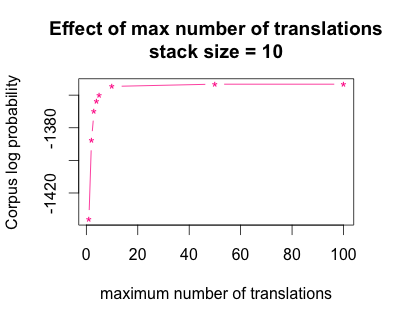
\includegraphics[scale=0.45]{d1_change_k.png}
		\caption{Increasing maximum number of translations, range [1-100].}
	\end{subfigure}
	\hskip2em
	\begin{subfigure}{.45\linewidth}
		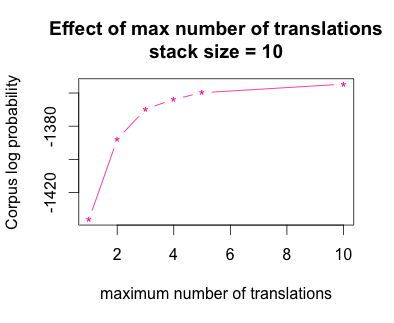
\includegraphics[scale=0.45]{d1_change_k_to10.png}
		\caption{Increasing maximum number of translations, range [1-10].}
	\end{subfigure}
	\hskip2em
	\begin{subfigure}{.45\linewidth}
		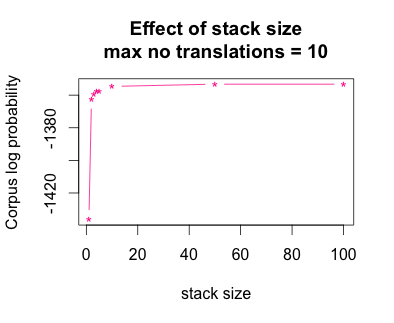
\includegraphics[scale=0.45]{d1_change_s.png}
		\caption{Increasing stack size, range [1-100].}
	\end{subfigure}
	\hskip2em
	\begin{subfigure}{.45\linewidth}
		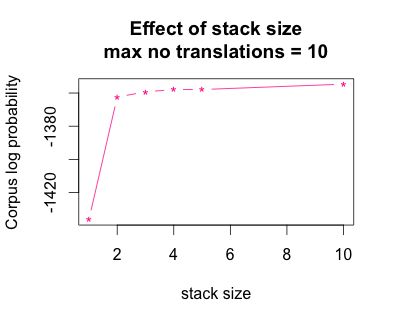
\includegraphics[scale=0.45]{d1_change_s_to10.png}
		\caption{Increasing stack size, range [1-10].}
	\end{subfigure}
	\caption{Performance of decoder without reordering - total corpus log probability as a function of maximum number of translations per phrase and stack size.}
\end{figure}

%----------------------------------------------------------------------------------------
%	Q 2
%----------------------------------------------------------------------------------------
\section*{Q2}
We modified the old $h(j,e)$ so that each recursion step reads two phrases
instead of one. The second of these phrases (in the French sentence) may be
the empty phrase $\varepsilon$. The two phrases are always swapped in the
translation. If the second phrase was $\varepsilon$, swapping has no effect
on the translation. Thus the translation is equivalent to a non-swap.
Our full definition of $h(j,e)$ is specified as follows:

$h (0 \nocomma, e) = \left\{ \begin{array}{l}
1 \nocomma, \tmop{if} \, e = \tmop{START}\\
0 \nocomma, \tmop{otherwise}
\end{array} \right.$
\begin{eqnarray}
h (j, e) = & \underset{h (i, e') e_1 \ldots e_k e_{k + 1} \ldots e_m
	e}{\tmop{argmax}}_{} & p (h (i, e')) \nonumber\\
& + & \log p_{\tmop{TM}} (f_{i + 1} \ldots f_c |e_{k + 1} \ldots e_m e)
\nonumber\\
& \noplus + & \log p_{\tmop{TM}} (f_{c + 1} \ldots f_j |e_1 \ldots e_k)
\nonumber\\
& \upl & \log p_{\tmop{LM}} (e_1 |e') + \sum_{k' = 1}^{m - 1} \log
p_{\tmop{LM}} (e_{k' + 1} |e_{k'}) + \log p_{\tmop{LM}} (e|e_m) \nonumber
\end{eqnarray}
with $0 \leq i < c \leq j$, $0 \leq k \leq m$, $e' \in V_E$, $e_1 \ldots e_k
\in t (f_{c + 1} \ldots f_j) \cup \{ \varepsilon \}$,\\
and $e_{k + 1} \ldots e_m e \in t (f_{i + 1} \ldots f_c)$.

python

%----------------------------------------------------------------------------------------
%	Q 3
%----------------------------------------------------------------------------------------
\section*{Q3}
For each French sentence of length $n$, we loop over all $n$ possible
stacks. In each stack, we look at the top $s$ hypotheses and expand them.
In each expansion, the algorithm contemplates all possible combinations of
the first $k$ translations of two French phrases, where it explores phrase
lengths of no more than $n$. Finally, the algorithm calculates the language
model probability of this combination. In this step, the algorithm has to
iterate over up to $2 t$ words, where $t$ is the maximum length of a
translation phrase. Thus the overall complexity is as follows:

\[
\mathcal{O}(n \cdot s) \cdot \mathcal{O}({(n \cdot k)}^2)
\cdot \mathcal{O}(t)
= \mathcal{O}(n^3 \cdot k^2 \cdot s \cdot t)
\]

%----------------------------------------------------------------------------------------
%	Q 4
%----------------------------------------------------------------------------------------
\section*{Q4}


%----------------------------------------------------------------------------------------
%	Q 5
%----------------------------------------------------------------------------------------
\section*{Q5}


%----------------------------------------------------------------------------------------
%	Q 6
%----------------------------------------------------------------------------------------
\section*{Q6}


\begin{figure}
	\centering
	\begin{subfigure}{.45\linewidth}
		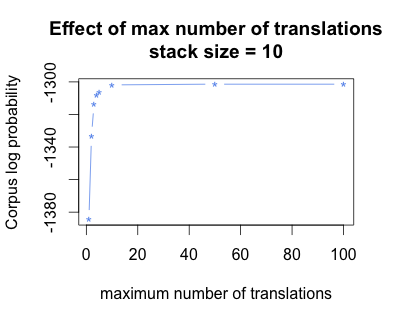
\includegraphics[scale=0.45]{d2_change_k.png}
		\caption{Increasing maximum number of translations, range [1-100].}
	\end{subfigure}
	\hskip2em
	\begin{subfigure}{.45\linewidth}
		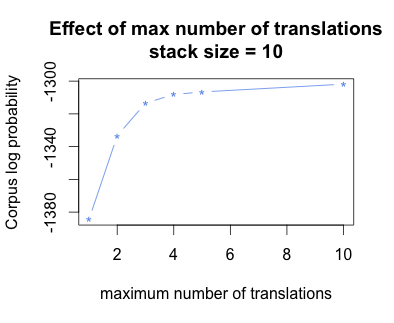
\includegraphics[scale=0.45]{d2_change_k_to10.png}
		\caption{Increasing maximum number of translations, range [1-10].}
	\end{subfigure}
	\hskip2em
	\begin{subfigure}{.45\linewidth}
		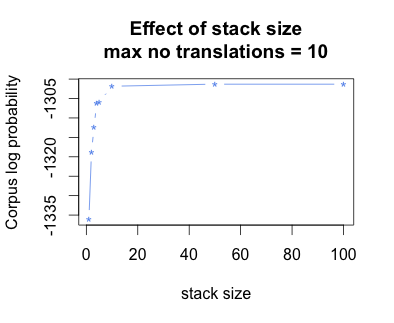
\includegraphics[scale=0.45]{d2_change_s.png}
		\caption{Increasing stack size, range [1-100].}
	\end{subfigure}
	\hskip2em
	\begin{subfigure}{.45\linewidth}
		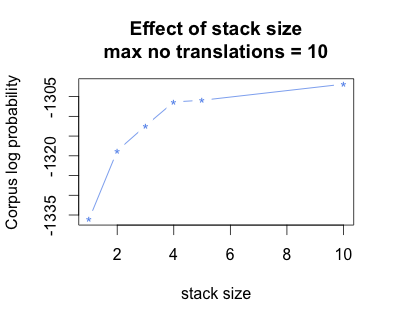
\includegraphics[scale=0.45]{d2_change_s_to10.png}
		\caption{Increasing stack size, range [1-10].}
	\end{subfigure}
	\caption{Performance of decoder with local reordering - total corpus log probability as a function of maximum number of translations per phrase and stack size.}
\end{figure}

%----------------------------------------------------------------------------------------
%	Q 7
%----------------------------------------------------------------------------------------
\section*{Q7}
We based our decoder on the correspondence between phrase-based decoding and the Traveling Salesmen Problem, following the proposal of \cite{zaslavskiy2009}.

Our implementation includes the following steps:
- create an asymmetric graph based on the French sentence, the translation model, and the English model;
- find the best path by utilizing the LKH package implementation of the Lin-Kernighan heuristic \cite{Helsgaun2006};

We transform a sentence into a asymmetric graph by following the procedure described in \cite{zaslavskiy2009}. We extract from the French sentence all phrases; for each phrase we retrieve all of its possible translations and for each of these we create a biphrase (French phrase, English translation). Then we create nodes of the graph by generating all possible pairs of a French word taken from the sentence and a biphrase of which this word is a part. Having crated all the nodes, we decide on the cost of each possible directed edge, again following the approach described in the article. We do not transform our graph to a symmetric one, since the TSP solver we use is capable of handling problems specified as asymmetric graphs.


%----------------------------------------------------------------------------------------
%	BIBLIOGRAPHY
%----------------------------------------------------------------------------------------
\bibliographystyle{apalike}

\bibliography{sample}

%----------------------------------------------------------------------------------------


\end{document}